%\documentclass[a4paper,10pt]{amsart}
\documentclass[a4paper,10pt]{article}
\usepackage[latin1]{inputenc}
\usepackage[spanish]{babel}
\spanishdecimal{.}
\usepackage[dvips]{epsfig}
\usepackage{graphicx}
\usepackage{verbatim}
\usepackage{amssymb}
\usepackage{amsmath}
\usepackage{amsfonts}

\title{Trabajo Pr\'actico Final\\ Simulaci\'on de Sistemas\\ (72.25)}

\author{
Abramowicz Pablo\\
Gomez Vidal Maximiliano\\
Sessa Carlos\\
Villa Fernandez Santiago\\
}

\begin{document}
\maketitle

\section*{Item A}

\subsection*{Tiempo entre arribos}


Para modelar el intervalo de tiempos entre arribos se cuenta con mediciones del
horario en que los clientes llegan al sistema. La regla de
Sturges para la elecci\'on de la cantidad de intervalos de clase 
aconseja utilizar $1 + \log_2 n$ intervalos, siendo $n$
la cantidad de datos. De esta manera se obtiene que se requieren $7.644$ intervalos,
utilizando en este caso $8$. 

\begin{figure*}[hp]
\centering
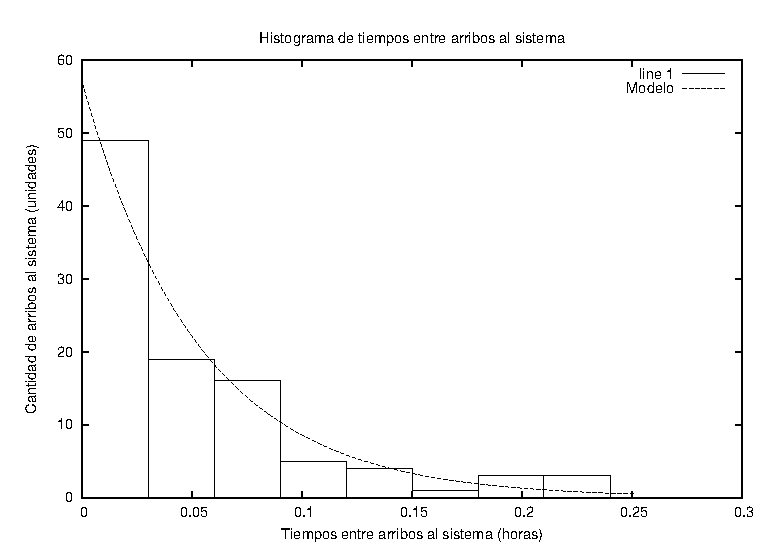
\includegraphics{graficos/histograma_llegadas.eps}
\caption{Tiempo entre arribos al sistema}
\label{fig:tiempoentrearribos}
\end{figure*}


En la figura ~\ref{fig:tiempoentrearribos} se observa el histograma con los
intervalos de tiempo entre arribos. Se percibe que los datos tienden a estar
distribuidos en forma exponencial. Se realiza un test de bondad de ajuste
$\chi^2$ para comprobarlo.


Se estima el valor medio de la muestra obteni\'endose 
$\lambda = 18.939$ [clientes/hora],
con un estad\'istico chi-cuadrado de valor $\chi_0^2 = 11.943$. 
El valor cr\'itico para $7$ grados de libertad con un nivel
de significaci\'on del $5\%$ resulta $\chi_{7,0.05}^2 = 14.067$. Por lo tanto,
no puede refutarse la hip\'otesis de que los datos provengan de una distribuci\'on 
exponencial.

\begin{figure*}[hp]
\centering
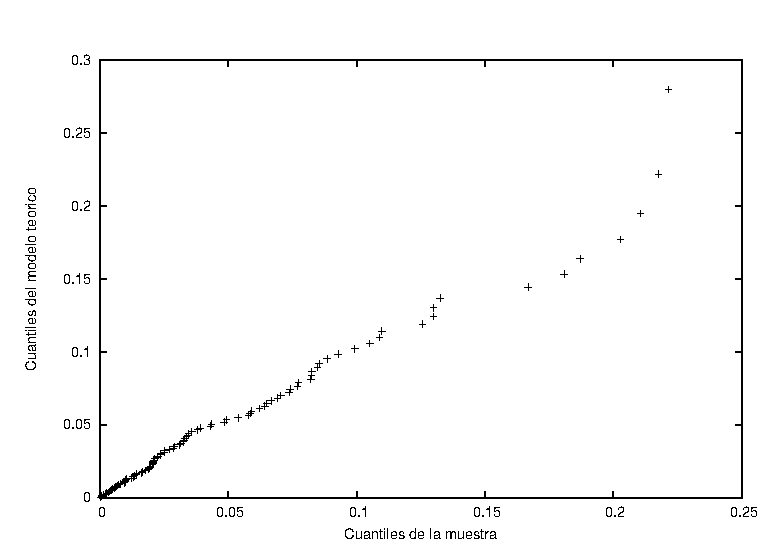
\includegraphics{graficos/plot_qq_llegadas.eps}
\caption{Plot Q-Q del tiempo entre arribos al sistema}
\label{fig:qqarribos}
\end{figure*}


En la figura ~\ref{fig:qqarribos} se muestra un plot Q-Q. Se visualiza que los cuantiles se encuentran
alineados sobre una recta de pendiente unitaria, en especial para valores
peque\~nos. De este an\'alisis se desprende que la distribuci\'on de la
muestra es muy similar a la exponencial.


Realizando un test de uniformidad
Kolmogorov-Smirnov sobre los tiempos de arribos se obtiene un estad\'istico
de $D = 0.12686$, considerando nuevamente los datos agrupados en $8$ clases. 
El valor cr\'itico para un nivel de significaci\'on del $5\%$ 
se obtiene de tabla y resulta $D_{7, 0.05} = 0.4361$.
Puesto que $D_{7,0.05} > D$ no se puede afirmar que los datos
no provengan de una distribuci\'on exponencial. 


Debido a que los tests resultaron satisfactorios, se supone para las 
simulaciones que los datos se encuentran distribuidos exponencialmente con media
$\lambda = 18.939$ [clientes/hora].


\subsection*{Tiempo de atenci\'on de la estaci\'on E3}


El resultado de aplicar la regla de Sturges indica utilizar $8.644$ intervalos
de clase. Empleando adem\'as la regla de Nu\~nez se opta por utilizar $8$ 
intervalos de clase.

\begin{figure*}[hp]
\centering
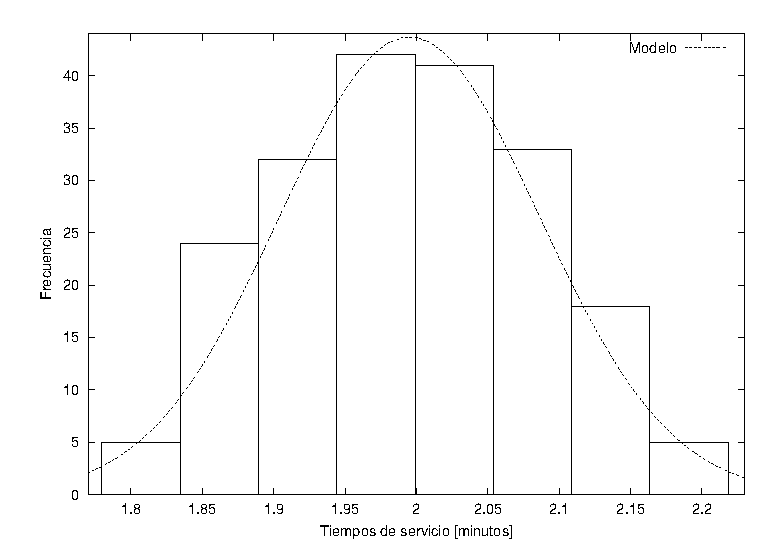
\includegraphics{graficos/histograma_e3.eps}
\caption{Tiempo de atenci\'on de la estaci\'on E3}
\label{fig:tiempoatencione3}
\end{figure*}


El histograma de tiempo de atenci\'on dado en la figura 
 ~\ref{fig:tiempoatencione3}
muestra que los datos presentan una distribuci\'on aproximadamente
normal.

La estimaci\'on de la media resulta $\mu = 1.9952 $ y la varianza tiene un valor
$\sigma^2 = 0.00832$. Se realiza el test de bondad de ajuste $\chi^2$ para
analizar si es razonable suponer que la distribuci\'on observada es normal.

\begin{figure*}[hp]
\centering
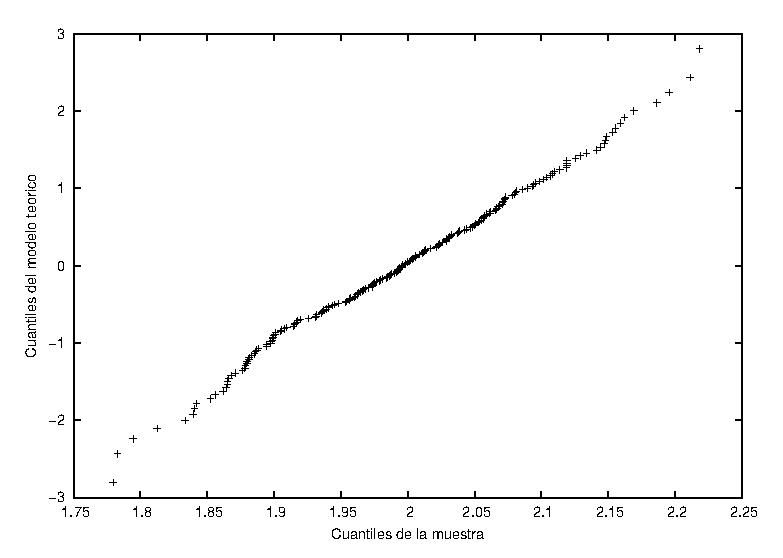
\includegraphics{graficos/plot_qq_e3.eps}
\caption{Plot Q-Q del tiempo de atenci\'on en la facilidad E3}
\label{fig:qqe3}
\end{figure*}


El valor del estad\'istico es $\chi_0^2 = 4.7492$, resultando menor que el valor 
cr\'itico obtenido por tablas para $7$ grados de libertad con un nivel de 
significaci\'on del $5\%$, cuyo valor es $\chi_{7,0.05}^2 = 14.067$. En
consecuencia, no se refuta la hip\'otesis de que los datos provengan de una 
distribuci\'on normal. En la figura  ~\ref{fig:qqe3} se observa el plot Q-Q comparando
ambas distribuciones.

\section*{Item B}

Todas las colas del sistema se modelan con capacidad infinita y un
comportamiento FIFO (\textit{first in- first out}), salvo la cola de la
facilidad $E3$, donde se considera que los clientes que no han llenado el
formulario son desplazados un lugar hacia atr\'as.


Las colas involucradas son $Q = \{R, E1, E3, OFT, PSF, E2, C\}$.


El estado del sistema puede ser completamente representado por la longitud
de cada una de las colas y el estado de las facilidades, ya sea
libre u ocupado. De esta forma, el espacio de estados resulta:

\begin{equation*}
\begin{split}
S = & \{(x_{R}, x_{E1}, x_{E3}, x_{OFT}, x_{PSF}, x_{E2}, x_{C}, s_{R},
s_{E1}, s_{E3}, s_{OFT}, s_{PSF}, s_{E2}, s_{C1}, s_{C2}, s_{C3}) / \\
& 
 x_{R}, x_{E1}, x_{E3}, x_{OFT}, x_{PSF}, x_{E2}, x_{C} = 0, 1, \dots \wedge \\
&
 s_{R},
s_{E1}, s_{E3}, s_{OFT}, s_{PSF}, s_{E2}, s_{C1}, s_{C2}, s_{C3} \in \{B, F\}\}
\end{split}
\end{equation*}

siendo $B$ el estado ocupado y $F$ el estado libre. 
Se considera tambi\'en que hay una \'unica cola para pagar, que cuenta con 3 
facilidades.

\section*{Item C}

Los eventos involucrados son la llegada y la salida de clientes a cada una 
de las colas. Adem\'as, debe considerarse cuando una facilidad comienza a 
atender a un cliente y cuando la misma finaliza el servicio.

El conjunto de eventos del sistema resulta entonces:

\begin{equation*}
\begin{split}
E = & \{R_a, R_d, E1_a, E1_d, E3_a, E3_d, OFT_a, OFT_d, PSF_a, PSF_d,
 E2_a, E2_d, C_a, C_d, \\
 & r_b, r_f, e1_b, e1_f, e3_b, e3_f, oft_b, oft_f,
 psf_b, psf_f, e2_b, e2_f, c1_b, c1_f, c2_b, c2_f, c3_b, c3_f \}
\end{split}
\end{equation*}


donde el sub\'indice $a$ indica la llegada de un cliente a la cola y el
sub\'indice $d$ indica la partida de un cliente de la cola.


Los eventos en min\'usculas se refieren a los cambios de estado de cada facilidad.
En el caso de empezar a atender un cliente se utiliza el sub\'indice $b$ y 
al finalizar de brindar el servicio el sub\'indice $f$.


Se considera que el tiempo de traslado de un cliente que ha sido atendido en
alguna facilidad hacia la pr\'oxima cola es nulo. Por lo tanto, resulta factible
simplificar el conjunto de eventos amalgamando aquellos que son
consecutivos sin bifurcaci\'{o}n posible. Por ejemplo, un cliente que finaliza
de abonar su recibo y se dirige a la estaci\'n E2 para retirar su registro
renovado.

\section*{Item D}

%TODO sacar la referencia al censo de aca y armar una nota al pie o algo de eso
En primer lugar se establecen las probabilidades de transici\'on entre estados.
Se supone que $5\%$ de las personas que se acercan a la recepci\'on solamente
desean obtener el instructivo. El resto desea efectuar el tr\'amite del
registro.


Se establece que el tiempo que tarda un cliente en llenar el formulario est\'a
distribuido de manera uniforme entre $3$ y $5$ minutos.


El $10\%$ de los que est\'an haciendo el tr\'amite
desean obtener el registro profesional, por lo que deber\'an presentarse
al test psico-f\'isico al igual que las personas mayores de $70$ a\~nos
(alrededor del $8\%$ de acuerdo al censo del $2000$).
Se considera que el $2\%$ desaprueba el test oftalmol\'ogico
o el test psico-f\'isico. 


El horario de atenci\'on los d\'ias h\'abiles es de $8.00$ a $13.00$. 
Inicialmente todas las colas se encuentran vac\'ias.
 

Para la simulaci\'on se utiliza la funci\'on \textit{rand} de 
\textit{GNU Octave 3.0.5}. La misma implementa el generador de n\'umeros
pseudo-aleatorios conocido como \textit{Twister de Mersenne}. Este generador
tiene un per\'iodo de $2^{19937} - 1$. Como semilla se define el n\'umero
$31337$.


De la figura  ~\ref{fig:colaR} a  ~\ref{fig:colaC} se observan las longitudes
de cada cola en funci\'on del tiempo. Como la velocidad de atenci\'on en las
facilidades R, E1 y C resulta bastante mayor que el ritmo al que llegan
clientes, las mismas permanecen ociosas la mayor parte de la jornada.
Se observan cuellos de botella en E2 y el test oftalmol\'ogico.

\begin{figure*}[hp]
\centering
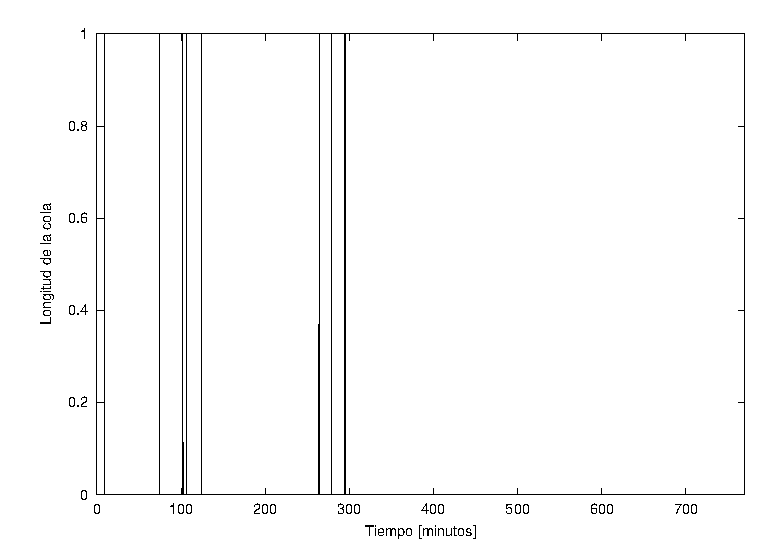
\includegraphics{graficos/plot_longitud_R.eps}
\caption{Longitud de la cola R}
\label{fig:colaR}
\end{figure*}

\begin{figure*}[hp]
\centering
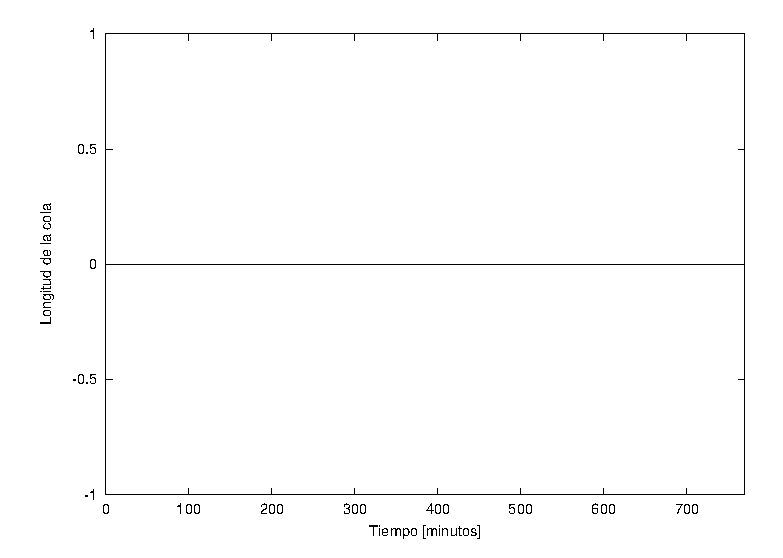
\includegraphics{graficos/plot_longitud_E1.eps}
\caption{Longitud de la cola E1}
\label{fig:colaE1}
\end{figure*}


\begin{figure*}[hp]
\centering
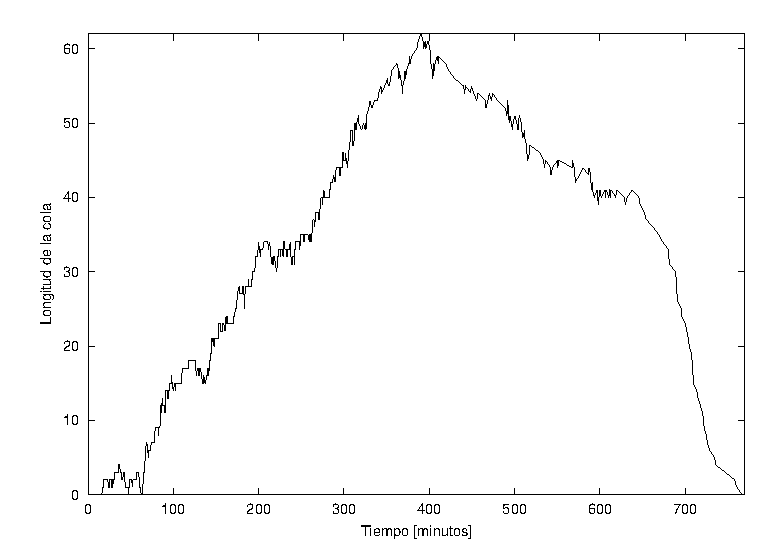
\includegraphics{graficos/plot_longitud_E2.eps}
\caption{Longitud de la cola E2}
\label{fig:colaE2}
\end{figure*}


\begin{figure*}[hp]
\centering
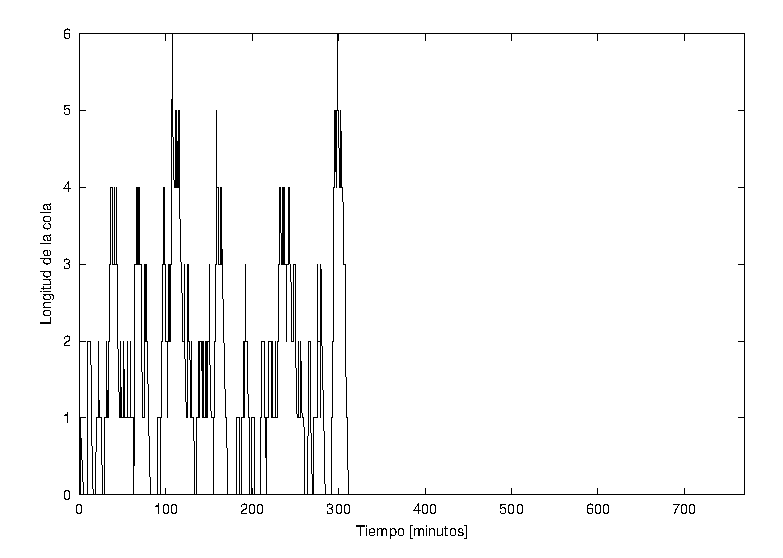
\includegraphics{graficos/plot_longitud_E3.eps}
\caption{Longitud de la cola E3}
\label{fig:colaE3}
\end{figure*}


\begin{figure*}[hp]
\centering
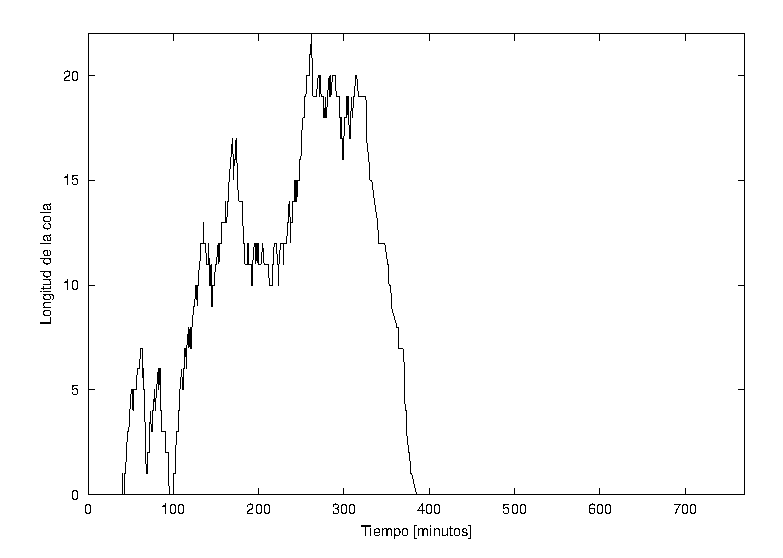
\includegraphics{graficos/plot_longitud_OFT.eps}
\caption{Longitud de la cola OFT}
\label{fig:colaOFT}
\end{figure*}


\begin{figure*}[hp]
\centering
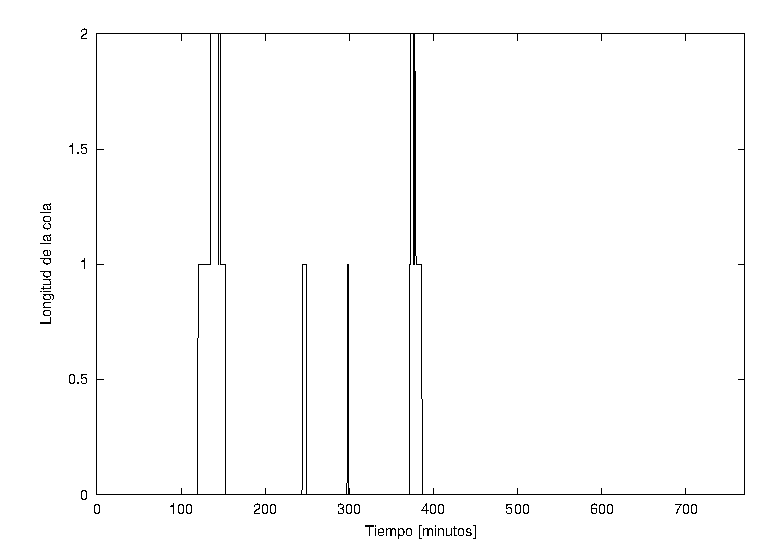
\includegraphics{graficos/plot_longitud_PSF.eps}
\caption{Longitud de la cola PSF}
\label{fig:colaPSF}
\end{figure*}


\begin{figure*}[hp]
\centering
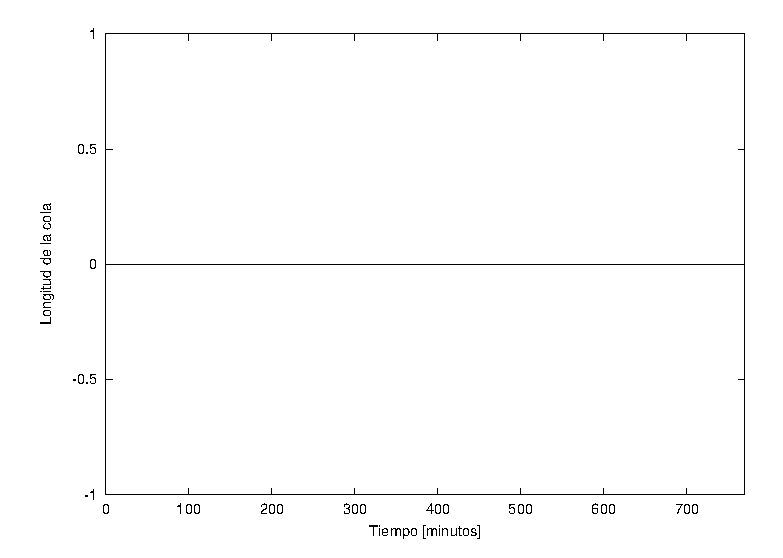
\includegraphics{graficos/plot_longitud_C.eps}
\caption{Longitud de la cola C}
\label{fig:colaC}
\end{figure*}

\section*{Item E}
Se realizan $10$ simulaciones independientes, utilizando para cada una el metodo de montecarlo con aproximadamente $1000$ iteraciones cada una.
En el cuadro $1$ se presenta la estimaci\'on de los tiempos medios junto con sus varianzas e intervalos de confianza ($\alpha = 0.01$).\\
\begin{table}
\begin{center}
\begin{tabular}{cccc} \hline \hline
N\'umero de simulaci\'on & Tiempo medio [minutos] & Varianza & Intervalo de confianza\\ \hline
\texttt{1}	& $276.62$ & $3991.30$ & $\pm3.92$\\
\texttt{2}	& $275.69$ & $3946.31$ & $\pm3.89$\\
\texttt{3}	& $275.68$ & $3910.77$ & $\pm3.88$\\
\texttt{4}	& $275.48$ & $3863.30$ & $\pm3.85$\\
\texttt{5}	& $275.31$ & $3928.56$ & $\pm3.88$\\
\texttt{6}	& $275.76$ & $3937.04$ & $\pm3.89$\\
\texttt{7}	& $275.88$ & $3954.88$ & $\pm3.90$\\
\texttt{8}	& $275.82$ & $3940.23$ & $\pm3.89$\\
\texttt{9}	& $276.09$ & $3943.13$ & $\pm3.89$\\
\texttt{10}	& $276.22$ & $3924.34$ & $\pm3.88$\\
\hline \hline
\end{tabular}
\end{center}
\label{tab:tiemposmedios}
\vspace{4pt}
\caption{Tiempo medio de un cliente en el sistema para 10 simulaciones
independientes.}
\end{table}

\section*{Item F}

En la figura ~\ref{fig:probac3} se muestra el tiempo medio de un cliente
en el sistema de acuerdo a la probabilidad de que la caja C3 se encuentre
operativa. Se observa que no se presentan grandes cambios en el tiempo medio.
Esto se debe a que la caja C3 est\'a libre la mayor parte del tiempo, puesto
que la tasa de llegada de clientes resulta inferior a la velocidad de atenci\'on
de las 3 cajas. En la figura ~\ref{fig:operativac3} se muestra este fen\'omeno.

\begin{figure*}[hp]
\centering
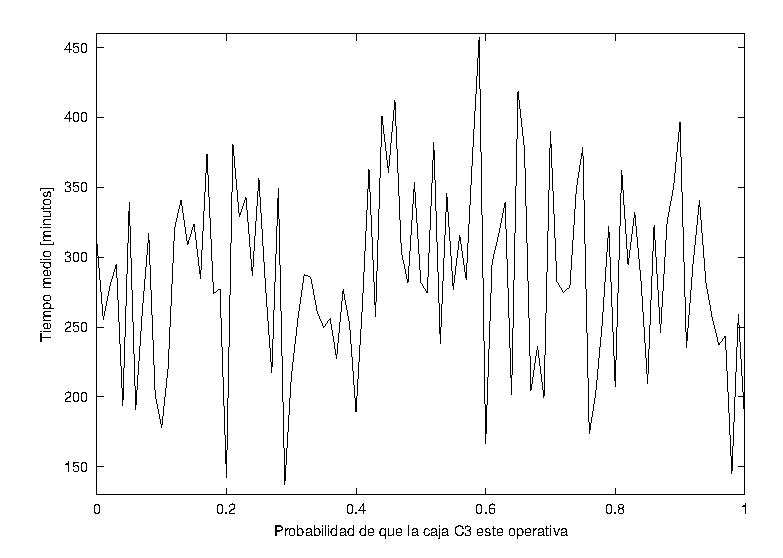
\includegraphics{graficos/plot_probabilidad_c3.eps}
\caption{Tiempo medio de un cliente en el sistema en funci\'on de la probabilidad
de que la caja C3 est\'e operativa}
\label{fig:probac3}
\end{figure*}


\begin{figure*}[hp]
\centering
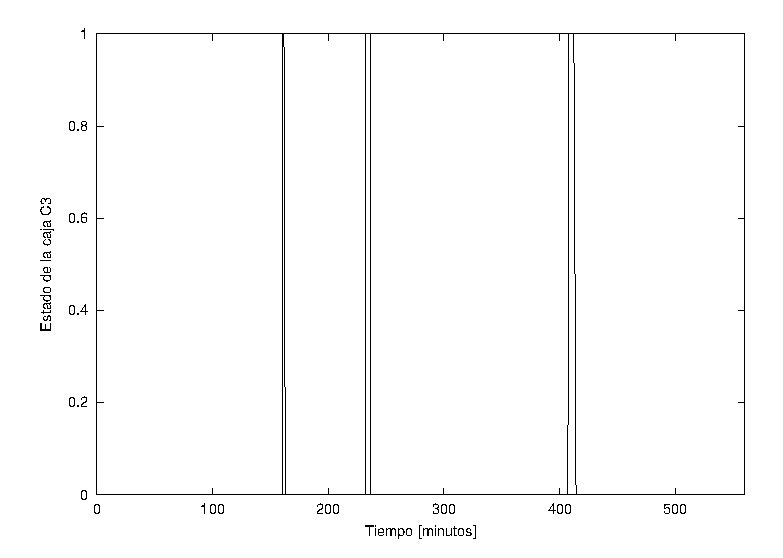
\includegraphics{graficos/plot_operatividad_c3.eps}
\caption{Estado de la caja C3 cuando se encuentra operativa durante toda la 
jornada}
\label{fig:operativac3}
\end{figure*}

\section*{Item G}

Se desea computar la probabilidad $p$ de que el tiempo medio de espera en la cola
OFT sea mayor a $5$ minutos. La estaci\'on OFT tarda $3.5$ minutos en promedio
para atender a un cliente.

Realizando 50 iteraciones con el m\'etodo de Montecarlo y fijando
como criterio de detenci\'on una variaci\'on menor a $0.000001$ entre dos iteraciones
sucesivas se obtiene $p = 0.7226 \pm 0.0599$ con un nivel de significaci\'on
del $5\%$. 


\end{document}
